\documentclass[addpoints]{exam}

\usepackage{amssymb, amsmath, amsfonts}
\usepackage{geometry}
\usepackage{graphicx}
\usepackage{tikz}
\usetikzlibrary{calc}
\usepackage{multirow,array} % for payoff matrix formatting
\usepackage[colorlinks,pdfusetitle,urlcolor=blue,citecolor=blue,linkcolor=blue]{hyperref}

\definecolor{crimson}{RGB}{ 170, 4, 36 }
\definecolor{darkblue}{RGB}{ 4, 47, 170 }
\definecolor{brown}{RGB}{ 111, 71, 2 }
\definecolor{periwinkle}{RGB}{ 90, 177, 204 }
\definecolor{ducksgreen}{HTML}{007030}

\geometry{left=1.0in,right=1.0in,top=1.0in,bottom=1.0in}
\pagestyle{headandfoot}
\lhead{EC327 Game Theory}
\chead{Homework 1}
\rhead{Winter 2024}
\runningheadrule

\title{
    \textbf{Econ 327: Game Theory} \\ 
    Homework $\#1$
    }
\author{University of Oregon}
\date{Due: Oct. 11$^{th}$}

% exam-type question formatting
\renewcommand{\thequestion}{\textbf{Question \arabic{question}}}
\bracketedpoints

\begin{document}

\maketitle

\begin{center}
  \gradetable[h][questions]
\end{center}

\vspace{0.5in}

\begin{center}
  \textbf{For homework assignments:}
\end{center}

\begin{itemize}

%  \item DO NOT write your name:
%  this assignment will be graded anonymously. 
%  If you want to, you can include your student ID instead.

  \item Complete \textit{all} questions and parts.
  % I will select one question at random to be graded
  % according to the rubric on Canvas.

  \item You may choose to work with others,
  but everyone must submit to Canvas individually.
  Please include the names of everyone who you worked with 
  below your own name.
 
\end{itemize}

\vspace{1.0in}

\makebox[.6\textwidth]{Name\enspace\hrulefill}

\vspace{0.5in}

% \begin{center}
%   \fbox{\fbox{\parbox{5.5in}{\centering
%     Answer the questions in the spaces provided on the
%     question sheets. If you run out of room for an answer,
%     continue on the back of the page or another sheet of paper.}}}
% \end{center}

\newpage

\begin{questions}

%------------------------------------------------------------------%

\question%[20]
\textbf{Multiple Choice}

\begin{parts}

  \part[4] 
  Which of the following is \textbf{not} an example of \textbf{strategic behavior}?
  \begin{choices}
    \CorrectChoice I always choose Chocolate over Vanilla ice cream because I like it better
    \choice More people bike on days with too much traffic
    \choice Apple markets \textit{Pro} versions of their products to people with money
    and non-Pro versions to broke students
    \choice Best Buy offer to match any competitors price offer for their customers
  \end{choices}

  \part[4] 
  \textbf{A}lice, \textbf{B}ob, and \textbf{C}onfucious 
  each put one dollar in a pot and each toss a fair coin.
  \textbf{A}lice wins if the coins are \textit{all heads} \textbf{or} \textit{all tails},
  \textbf{B}ob wins if there are \textit{2 heads} and \textit{1 tail},
  and \textbf{C}onfucious wins if there are \textit{1 head} and \textit{2 tails}.

  What are the \textbf{expected payoffs} for each player? 
  \footnote{Adapted from Dixit, Skeath, \& McAdams (2021)}
  \begin{choices}
    \choice $EU_A = \$0$,  $EU_B = \$0$,  $EU_C = \$0$ 
    \CorrectChoice $EU_A = -\$0.25$,  $EU_B = \$0.125$,  $EU_C = \$0.125$ 
    \choice $EU_A = -\$0.50$,  $EU_B = \$0.25$,  $EU_C = \$0.25$ 
    \choice $EU_A = \$0.50$,  $EU_B = -\$0.25$,  $EU_C = -\$0.25$
  \end{choices}

  \part[4] Consider the game tree below
  \begin{figure}[!h]
    \centering
    % macro for inputting terminal nodes
\newcommand\term[2]{\node[below]at(#1){$#2$};}
%
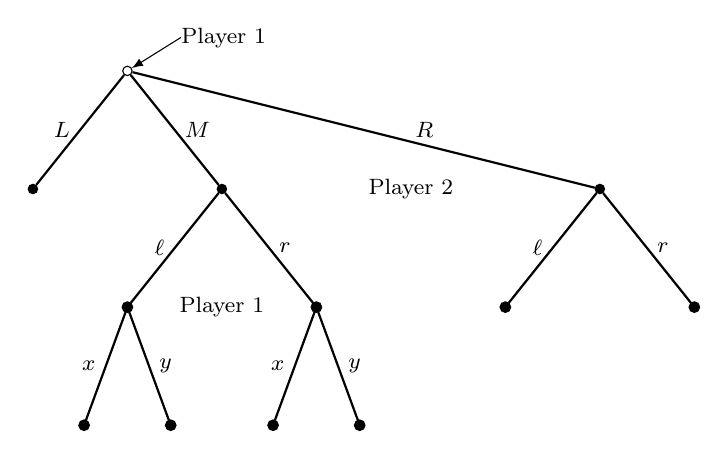
\begin{tikzpicture}[font=\footnotesize,edge from parent/.style={draw,thick}]
% Two node styles: solid and hollow
\tikzstyle{solid node}=[circle,draw,inner sep=1.2,fill=black];
\tikzstyle{hollow node}=[circle,draw,inner sep=1.2];
% Specify spacing for each level of the tree
\tikzstyle{level 1}=[level distance=15mm,sibling distance=12mm]
\tikzstyle{level 2}=[level distance=15mm,sibling distance=24mm]
\tikzstyle{level 3}=[level distance=15mm,sibling distance=11mm]
% The Tree
\node(0)[hollow node]{}
child{node[solid node]{}edge from parent node[left]{$L$}}
child{node[solid node]at +(\tikzsiblingdistance,0){}
child{node[solid node]{}
child{node[solid node]{}edge from parent node[left]{$x$}}
child{node[solid node]{}edge from parent node[right]{$y$}}
edge from parent node[left]{$\ell$}
}
child{node[solid node]{}
child{node[solid node]{}edge from parent node[left]{$x$}}
child{node[solid node]{}edge from parent node[right]{$y$}}
edge from parent node[right]{$r$}
}
edge from parent node[right]{$M$}
}
child[sibling distance=5*\tikzsiblingdistance]{node[solid node]{}
child{node[solid node]{}
edge from parent node[left]{$\ell$}
}
child{node[solid node]{}
edge from parent node[right]{$r$}
}
edge from parent node[right,xshift=15]{$R$}
};
% specifying movers
\draw[draw,<-,>=latex](0)--(32:8mm)node[right,inner sep=0]{Player 1};
\node at ($.5*(0-2)+.5*(0-3)$) {Player 2};
\node at ($.5*(0-2-1)+.5*(0-2-2)$) {Player 1};
\end{tikzpicture}

  \end{figure}

  (recall that a strategy is a complete plan of action
  for \textit{every} eventuality)

  Which of the following is a \textbf{complete strategy for Player 1}?
  \begin{choices}
    \choice ($L$)
    \choice ($x$ if $\ell$)
    \CorrectChoice ($L$, $x$ if $\ell$, $y$ if $r$)
    \choice ($R$) 
  \end{choices}

  \part[4] Consider the game tree from the previous question.

  Which of the following is a \textbf{complete strategy for Player 2}?
  \begin{choices}
    \choice ($\ell$ if $M$)
    \choice ($r$ if $M$, $\ell$ if $R$)
    \choice ($\ell$)
    \choice ($\ell$ if \L, $r$ if $M$, $r$ if $R$)
  \end{choices}

  \newpage

  \part[4] Consider the game tree below
  \begin{figure}[!h]
    \centering
    % example from: https://www.sfu.ca/~haiyunc/notes/Game_Trees_with_TikZ.pdf

\begin{tikzpicture}[scale=1.5,font=\footnotesize]
    \tikzstyle{solid node}=[circle,draw,inner sep=1.5,fill=black]
    \tikzstyle{hollow node}=[circle,draw,inner sep=1.5]
    \tikzstyle{level 1}=[level distance=15mm,sibling distance=3.5cm]
    \tikzstyle{level 2}=[level distance=15mm,sibling distance=1.5cm]
    \tikzstyle{level 3}=[level distance=15mm,sibling distance=1cm]
    
    \node(0)[solid node,label=above:{$P1$}]{}
        child{node[solid node,label=above left:{$P2$}]{}
            child{node[hollow node,label=below:{$(2,2)$}]{} edge from parent node[left]{$C$}}
            child{node[hollow node,label=below:{$(2,-1)$}]{} edge from parent node[left]{$D$}}
            child{node[hollow node,label=below:{$(3,1)$}]{} edge from parent node[right]{$E$}}
            edge from parent node[left,xshift=-5]{$A$}
        }
        child{node[solid node,label=above right:{$P2$}]{}
            child{node[hollow node,label=below:{$(2,2)$}]{} edge from parent node[left]{$F$}}
            child{node[hollow node,label=below:{$(1,3)$}]{} edge from parent node[right]{$G$}}
            edge from parent node[right,xshift=5]{$B$}
        };
\end{tikzpicture}

  \end{figure}
  Find the \textbf{rollback equilibrium}.
  \begin{choices}
    \choice \textbf{P1:} ($A$), \textbf{P2:} ($C$ if $A$, $F$ if $B$)
    \CorrectChoice \textbf{P1:} ($A$), \textbf{P2:} ($C$ if $A$, $G$ if $B$)
    \choice \textbf{P1:} ($B$), \textbf{P2:} ($C$ if $A$, $F$ if $B$)
    \choice \textbf{P1:} ($B$), \textbf{P2:} ($D$ if $A$, $G$ if $B$)
  \end{choices}

  \part[4] Consider the following variation to the Survivor Flags game: 

  There are 100 flags to start with, two teams who take turns taking flags,
  each team can take any number of flags between 1 and 10 on their turn,
  and the team to take the last flag wins.

  How many flags should the first team take?
  \begin{choices}
    \CorrectChoice 1
    \choice 2
    \choice 5
    \choice 10
  \end{choices}

  \part[4] \textbf{Rationality} means that:
  \begin{choices}
    \choice Players have perfect information
    \choice Players never make mistakes
    \choice Players have perfect recall
    \CorrectChoice Preferences are complete and transitive
  \end{choices}

\end{parts}

\newpage

%------------------------------------------------------------------

\question%[20]
Imagine a sequential moves version of rock-paper-scissors
where player 2 gets to pick what they will do after player 1 picks.
Please model the game in its extensive form (as a game tree). 
Assume both player 1 and player 2 only care about the result of the game
and have the following preferences over the result of the game:
win $\succ$ tie $\succ$ loss.
\footnote{Ethan Holdahl, University of Oregon }

\begin{parts}
 
  \part Answer the following questions:
  \begin{subparts}
    \subpart[4] How many nodes are there?
    \subpart[4] How many branches are there?
    \subpart[4] How many terminal nodes are there?
  \end{subparts}

  \part[10] Prune the tree as much as possible. How many branches were you able to eliminate?
    (A complete answer should include your drawing(s) of the game tree)

  \part[10]
  Use the same setup, but now imagine player 1's preferences change
  because they want to be seen as a "tough guy".
  Given that what they want to play remains the same,
  they still have the following preferences over the result of the game:
  win $\succ$ tie $\succ$ loss.
  However, they now would prefer to lose playing rock
  than win playing paper or scissors. 
  Please create a new game tree so the payoffs reflect these new preferences.

  Prune the tree as much as possible. 

  How many branches were you able to eliminate?
    (Include your drawing(s))

\end{parts}

\begin{solution}
\begin{parts}

  \part
  \begin{center}[!h]
    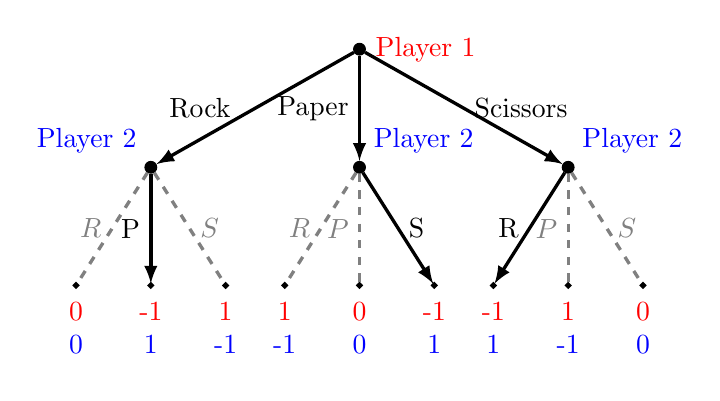
\begin{tikzpicture}[edge from parent/.style={draw, very thick, -latex}]
    \tikzstyle{solid node}=[circle,draw,inner sep=1.5,fill=black]
    \tikzstyle{hollow node}=[circle,draw,inner sep=.25]
    \tikzstyle{level 1}=[level distance=15mm,sibling distance=2.65cm]
    \tikzstyle{level 2}=[level distance=15mm,sibling distance=.95cm]
    \tikzstyle{level 3}=[level distance=15mm,sibling distance=.6cm]
    \tikzstyle{pruned edge from parent}=[draw, very thick, gray, dashed, -]
    
    \node(0)[solid node,label=right:{\color{red} Player 1}]{}
        child{node(1)[solid node,label=above left:{\color{blue} Player 2 }]{}
            child{node[hollow node,label=below:{
                \begin{tabular}{c}
                     {\color{red} 0}  \\
                     {\color{blue} 0} 
                \end{tabular}
            }]{} edge from parent[draw, very thick, gray, dashed, -] node[left]{$R$}}
            child{node[hollow node,label=below:{
                \begin{tabular}{c}
                     {\color{red} -1}  \\
                     {\color{blue} 1} 
                \end{tabular}
            }]{} edge from parent node[left]{P}}
            child{node[hollow node,label=below:{
                \begin{tabular}{c}
                     {\color{red} 1}  \\
                     {\color{blue} -1} 
                \end{tabular}
            }]{} edge from parent[draw, very thick, gray, dashed, -] node[right]{$S$}}
            edge from parent node[left,xshift=-5]{Rock}
        }
        child{node(2)[solid node,label=above right:{\color{blue} Player 2 }]{}
            child{node[hollow node,label=below:{
                \begin{tabular}{c}
                     {\color{red} 1}  \\
                     {\color{blue} -1} 
                \end{tabular}
            }]{} edge from parent[draw, very thick, gray, dashed, -] node[left]{$R$}}
            child{node[hollow node,label=below:{
                \begin{tabular}{c}
                     {\color{red} 0}  \\
                     {\color{blue} 0} 
                \end{tabular}
            }]{} edge from parent[draw, very thick, gray, dashed, -] node[left]{$P$}}
            child{node[hollow node,label=below:{
                \begin{tabular}{c}
                     {\color{red} -1}  \\
                     {\color{blue} 1} 
                \end{tabular}
            }]{} edge from parent node[right]{S}}
            edge from parent node[left]{Paper}
        }
        child{node(3)[solid node,label=above right:{\color{blue} Player 2 }]{}
            child{node[hollow node,label=below:{
                \begin{tabular}{c}
                     {\color{red} -1}  \\
                     {\color{blue} 1} 
                \end{tabular}
            }]{} edge from parent node[left]{R}}
            child{node[hollow node,label=below:{
                \begin{tabular}{c}
                     {\color{red} 1}  \\
                     {\color{blue} -1} 
                \end{tabular}
            }]{} edge from parent[draw, very thick, gray, dashed, -] node[left]{$P$}}
            child{node[hollow node,label=below:{
                \begin{tabular}{c}
                     {\color{red} 0}  \\
                     {\color{blue} 0} 
                \end{tabular}
            }]{} edge from parent[draw, very thick, gray, dashed, -] node[right]{$S$}}
            edge from parent node[right]{Scissors}
        };
\end{tikzpicture}

  \end{center}
  
  In the figure, dashed lines represent those which have been pruned.

  The tree has 4 nodes, 12 branches, and 9 terminal nodes.

  \part
  In each of Player 2's subgames,
  we can prune the two branches where they would lose or tie
  based on what Player 1 chose.
  We can't prune any more branches
  because Player 1 is indifferent between all outcomes where they lose.

  \part
  \begin{center}[!h]
    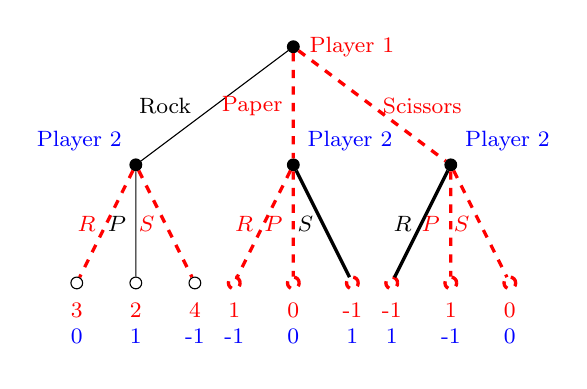
\begin{tikzpicture}[font=\footnotesize]
    \tikzstyle{solid node}=[circle,draw,inner sep=1.5,fill=black]
    \tikzstyle{hollow node}=[circle,draw,inner sep=1.5]
    \tikzstyle{level 1}=[level distance=15mm,sibling distance=2cm]
    \tikzstyle{level 2}=[level distance=15mm,sibling distance=.75cm]
    \tikzstyle{level 3}=[level distance=15mm,sibling distance=.5cm]
    
    \node(0)[solid node,label=right:{\color{red} Player 1}]{}
        child{node(1)[solid node,label=above left:{\color{blue} Player 2 }]{}
            child{node[hollow node,label=below:{
                \begin{tabular}{c}
                     {\color{red} 3}  \\
                     {\color{blue} 0} 
                \end{tabular}
            }]{} edge from parent[red, dashed, very thick] node[left]{$R$}}
            child{node[hollow node,label=below:{
                \begin{tabular}{c}
                     {\color{red} 2}  \\
                     {\color{blue} 1} 
                \end{tabular}
            }]{} edge from parent node[left]{$P$}}
            child{node[hollow node,label=below:{
                \begin{tabular}{c}
                     {\color{red} 4}  \\
                     {\color{blue} -1} 
                \end{tabular}
            }]{} edge from parent[red, dashed, very thick] node[left]{$S$}}
            edge from parent node[left,xshift=-5]{Rock}
        }
        child{node(2)[solid node,label=above right:{\color{blue} Player 2 }]{}
            child{node[hollow node,label=below:{
                \begin{tabular}{c}
                     {\color{red} 1}  \\
                     {\color{blue} -1} 
                \end{tabular}
            }]{} edge from parent[red, dashed, very thick] node[left]{$R$}}
            child{node[hollow node,label=below:{
                \begin{tabular}{c}
                     {\color{red} 0}  \\
                     {\color{blue} 0} 
                \end{tabular}
            }]{} edge from parent[red, dashed, very thick] node[left]{$P$}}
            child{node[hollow node,label=below:{
                \begin{tabular}{c}
                     {\color{red} -1}  \\
                     {\color{blue} 1} 
                \end{tabular}
            }]{} edge from parent[black, solid] node[left]{$S$}}
            edge from parent[red, dashed, very thick] node[left]{Paper}
        }
        child{node(3)[solid node,label=above right:{\color{blue} Player 2 }]{}
            child{node[hollow node,label=below:{
                \begin{tabular}{c}
                     {\color{red} -1}  \\
                     {\color{blue} 1} 
                \end{tabular}
            }]{} edge from parent[black, solid] node[left]{$R$}}
            child{node[hollow node,label=below:{
                \begin{tabular}{c}
                     {\color{red} 1}  \\
                     {\color{blue} -1} 
                \end{tabular}
            }]{} edge from parent[red, dashed, very thick] node[left]{$P$}}
            child{node[hollow node,label=below:{
                \begin{tabular}{c}
                     {\color{red} 0}  \\
                     {\color{blue} 0} 
                \end{tabular}
            }]{} edge from parent[red, dashed, very thick] node[left]{$S$}}
            edge from parent[red, dashed, very thick] node[right]{Scissors}
        };
\end{tikzpicture}

  \end{center}

  I represented Player 1's preferences as:

  payoff to winning with rock = 4,
  tie with rock = 3, 
  lose with rock = 2,
  win with paper or scissors = 1,
  tie with paper or scissors = 0,
  lose with paper or scissors = -1.

  Because payoffs are \textit{ordinal}, 
  you can choose any values as long as the ranking is the same.

  Now because Player 1 prefers to lose with rock to any other loss, 
  we can prune the branches where they choose either 
  paper or scissors.
  
  The rollback solution is 
  \{ Player 1 chooses Rock, 
  (Player 2 chooses paper if rock,
  scissors if paper,
  and rock if scissors) \}.

  \noindent\rule[0.5ex]{\linewidth}{1pt}
   
  \textbf{Grading:}

  This question is worth 20 points total, 
  with 10 for correctness, 5 for format, and 5 for explanation.

  \begin{itemize}
  \item 
  For part a, each correct number is worth 1 point.

  \item
  For part b, give 1 point if the overall structure is there,
  1 point if the payoffs go to the right node, 
  and 1 point if the correct 6 branches are pruned and no others.
  
  \item
  For part a on the second page (sorry), 
  give 1 correctness point for every correctly pruned branch,
  with -1 point for pruning other branches.
  \end{itemize}

  Scores for formatting and explanation are left up to the grader's interpretation of the rubric.

\end{parts}
\end{solution}

\newpage

%------------------------------------------------------------------

\question%[20]

Read the 2022 Policito Opinion article, 
\textit{How Game Theory Explains Why We Have to Sanction Putin : Even If It’s Costly}.

\url{https://www.politico.com/news/magazine/2022/04/21/russia-sanctions-game-theory-00026566}

\begin{parts}

  \part[8]
  List the tools from game theory that we've learned about in class
  which the authors use to argue their point.

  \part[10] 
  What assumptions do they make in their simplified model 
  of international sanctions?

  \part[10]
  Choose one assumption of the author's model to change 
  and explain how it changes what the model predicts.

\end{parts}

%------------------------------------------------------------------

% \question%[20]
% Here's a little ditty, about Jack and Diane,
% two American kids growing up in the heartland.
% The game is below.
% \footnote{Cliff Bekar, Lewis and Clark College}
%
%   \begin{table}[h!]
%     \centering
%     \setlength{\extrarowheight}{2pt}
%     \begin{tabular}{*{5}{c|}}
%       \multicolumn{2}{c}{} & \multicolumn{3}{c}{Diane} \\\cline{3-5}
%       \multicolumn{1}{c}{} &     & $x$ & $y$ & $z$ \\\cline{2-5}
%       \multirow{3}*{Jack}  & $a$ & 1,1 & 2,1 & 2,0 \\\cline{2-5}
%                            & $b$ & 2,3 & 0,2 & 2,1 \\\cline{2-5}
%                            & $c$ & 2,1 & 1,2 & 3,0 \\\cline{2-5}
%     \end{tabular}
%   \end{table}
%
% \begin{parts}
%   \part[8] Find all pure Nash strategy profiles and outcomes 
%     if Jack and Diane move simultaneously.
%     Carefully detail and explain your strategy profiles 
%     and how they map onto your Nash outcomes. 
%     \part[12] Find all pure Nash strategy profiles and outcomes
%     if Jack moves first.
%     Carefully detail and explain your strategy profiles 
%     and how they map onto your Nash outcomes.
% \end{parts}
%
% \begin{solution}
%   \begin{parts} 
%     \part Players: $\{ \text{Jack, Diane} \}$
%
%     Strategy sets: $S_{\text{Jack}} = \{ a, b, c \}$
%     $S_{\text{Diane}} = \{ x, y, c \}$
%
%     For Jack, $b$ and $c$ are best responses to $x$,
%     $a$ is BR to $y$,  
%     and $c$ is BR to $z$.
%
%     For Diane, $x$ and $y$ are BR to $a$,
%     $x$ is BR to $b$,
%     and $z$ is BR to $c$.
%
%     There are two strategy profiles where each player's best responses intersect:
%
%     \begin{itemize}
%       \item $N_1 = \{ b, x \}$ 
%
%       Jack's strategy is to choose $b$, 
%       Diane's strategy is to choose $x$.
%       Neither have regrets about their strategy choice;
%       given that Jack is choosing $b$, Diane can't get a higher payoff by deviating.
%       Given that Diane is playing $x$, Jack is indifferent between playing $b$ and $c$ but he can't get a strictly higher payoff by deviating. 
%       The resulting outcome is that Jack gets $2$, 
%       Diane gets $3$.
%
%       \item $N_2 = \{ a, y \}$
%
%       Jack's strategy is $a$, Diane's is $y$. 
%       When Jack plays $a$, Dianne is indifferent between $x$ and $y$, but
%       still cannot deviate to a strictly higher payoff.
%       When Diane plays $y$, Jack's best response is $a$ because $2>\{0,1\}$. 
%       The outcome is that Jack gets $2$ and Diane gets $1$.
%
%     \end{itemize}
%
%     These are the only two \textit{pure strategy} Nash equilibria
%     because there are no other intersections of pure strategy best responses.
%     Note that even though $N_1$ Pareto dominates $N_2$ 
%     (Jack is indifferent; $2=2$, and Diane is better off; $3>1$),
%     there is no \textit{unilateral} deviation that would reach $N_1$
%     from $N_2$.
%
%
%     \part
%     See the extensive form game tree below.
%
%     Now the strategy sets are: 
%
%     $S_{\text{Jack}} = \{ a, b, c \}$
%     because Jack still has only one decision node.
%
%     $S_{\text{Diane}} = \{$ any combination $ c_1 c_2 c_3$ where $c$ can be either $x$, $y$, or $z \}$
%     because Diane now has 3 elements in her information set.
%     She knows whether Jack has chosen $a$, $b$, or $c$ before she makes her own choice. 
%
%     I represented each of Diane's strategies as a triple where the first letter represents her choice at node 1, second letter at node 2, and third letter at node 3.
%     So for example, $xyz$ would be the strategy where she chooses $x$ in node $1$, $y$ in node $2$, and $z$ in node $3$. 
%
%     \begin{itemize}
%
%       \item 
%       $\mathbf{N_1} = \{ a, \ yc_2c_3 | 
%       \text{where $c_2$ is $x$, $y$, or $z$;
%       $c_3$ is $x$ or $y$ } \}$
%
%       Any set of strategies in which Jack chooses $a$
%       and Diane chooses $y$ in node $1$ 
%       but doesn't choose $z$ at node $3$
%       would result in an equilibrium outcome of 
%       $({\color{red} 2},{\color{blue} 1})$
%       where Jack cannot deviate to a higher payoff than $2$,
%       and Diane also has no regrets with choosing $y$.
%
%       \item 
%       $\mathbf{N_2} = \{ b, \ xc_2c_3 |
%       \text{where $c_2$ could be $x$, $y$, or $z$;
%       $c_3$ could be either $x$ or $y$ }\}$
%
%       Any set of strategies in which Jack chooses $b$ 
%       and Diane doesn't choose $z$ at node $3$ 
%       would result in Jack choosing $b$ 
%       and Diane choosing $x$ given that jack chooses $b$. 
%
%       The equilibrium outcome of any of these Nash strategy profiles
%       would be $({\color{red} 2}, {\color{blue} 3})$
%
%     \end{itemize}
%
%   \end{parts}
%
% \begin{center}
%   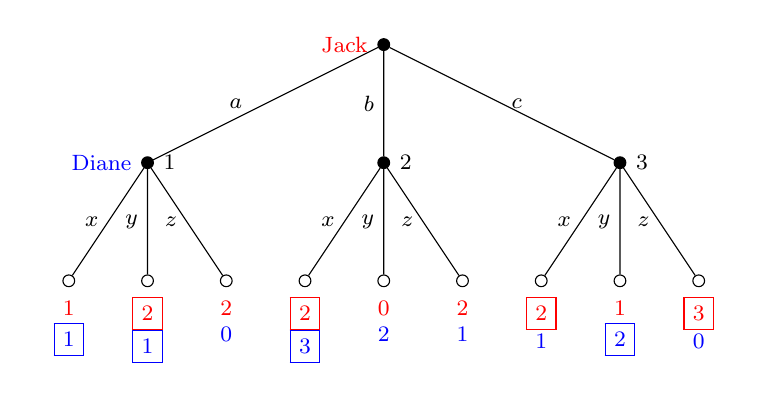
\begin{tikzpicture}[font=\footnotesize]
    \tikzstyle{solid node}=[circle,draw,inner sep=1.5,fill=black]
    \tikzstyle{hollow node}=[circle,draw,inner sep=1.5]
    \tikzstyle{level 1}=[level distance=15mm,sibling distance=3cm]
    \tikzstyle{level 2}=[level distance=15mm,sibling distance=1cm]
    \tikzstyle{level 3}=[level distance=15mm,sibling distance=.5cm]
    
    \node(0)[solid node,label=left:{\color{red} Jack}]{}
        child{node(1)[solid node,label=left:{\color{blue} Diane },label=right:{$1$}]{}
            child{node[hollow node,label=below:{
                \begin{tabular}{c}
                     {\color{red} 1}  \\
                     {\color{blue} \boxed{1}} 
                \end{tabular}
            }]{} edge from parent[] node[left]{$x$}}
            child{node[hollow node,label=below:{
                \begin{tabular}{c}
                  {\color{red} \boxed{2}}  \\
                     {\color{blue} \boxed{1}} 
                \end{tabular}
            }]{} edge from parent node[left]{$y$}}
            child{node[hollow node,label=below:{
                \begin{tabular}{c}
                     {\color{red} 2}  \\
                     {\color{blue} 0} 
                \end{tabular}
            }]{} edge from parent[ ] node[left]{$z$}}
            edge from parent node[left,xshift=-5]{$a$}
        }
        child{node(2)[solid node,label=right:{$2$}]{}
            child{node[hollow node,label=below:{
                \begin{tabular}{c}
                  {\color{red} \boxed{2}}  \\
                     {\color{blue} \boxed{3}} 
                \end{tabular}
            }]{} edge from parent[] node[left]{$x$}}
            child{node[hollow node,label=below:{
                \begin{tabular}{c}
                     {\color{red} 0}  \\
                     {\color{blue} 2} 
                \end{tabular}
            }]{} edge from parent[ ] node[left]{$y$}}
            child{node[hollow node,label=below:{
                \begin{tabular}{c}
                     {\color{red} 2}  \\
                     {\color{blue} 1} 
                \end{tabular}
            }]{} edge from parent[ ] node[left]{$z$}}
            edge from parent node[left]{$b$}
        }
        child{node(3)[solid node,label=right:{$3$}]{}
            child{node[hollow node,label=below:{
                \begin{tabular}{c}
                  {\color{red} \boxed{2}}  \\
                     {\color{blue} 1} 
                \end{tabular}
            }]{} edge from parent[ ] node[left]{$x$}}
            child{node[hollow node,label=below:{
                \begin{tabular}{c}
                     {\color{red} 1}  \\
                     {\color{blue} \boxed{2}} 
                \end{tabular}
            }]{} edge from parent[] node[left]{$y$}}
            child{node[hollow node,label=below:{
                \begin{tabular}{c}
                  {\color{red} \boxed{3}}  \\
                     {\color{blue} 0} 
                \end{tabular}
            }]{} edge from parent[ ] node[left]{$z$}}
            edge from parent node[right]{$c$}
        };
\end{tikzpicture}

% \end{center}
%
% \end{solution}
%
% \newpage
%
%
%------------------------------------------------------------------

% \question%[20]
% See the figures below for the data from our in-class activity 2 
% \footnote{You can also find the data on Canvas in the \textit{Activities} folder of the \textit{files} tab}.
% where teams took turns taking flags from a starting pool. 
% Note that in Game 1,
% 6 out of 9 matches were won by the first team to take flags 
% and in Game 2, 3 of 9 matches were won by the starting team.
%
% \begin{parts}
%   \part[10] Using the rollback equilibrium as a predictive model,
%   how many times would you expect the starting team to win 
%   when all agents are \textit{perfectly informed}, \textit{rational},
%   and have \textit{common knowledge of rationality}?
%   Based on the class data, should we \textit{accept} or \textit{reject}
%   this hypothesis?
%
%   \part[10] Based on your observations in class 
%   and the results from other groups, 
%   which of the assumptions above do you think could be modified
%   to create a more accurate model of this game?
%   What modifications would you make,
%   and what alternative hypotheses could you test?
%
% \end{parts}
%
% \begin{solution}
%   \begin{parts}
%
%     \part 
%     The first team can win 100\% of the time by always leaving a multiple of 
%     the maximum flags which can be taken plus one. 
%     So if all teams know the rules of the game then we would predict that
%     100\% of matches will be won by the starting team.
%
%     However, in class only 9 out of 18 matches were won by the starting team. 
%     We can pretty easily reject the 100\% win hypothesis.
%
%     \part 
%     This one is open to interpretation.
%     It might be that not everyone was fully paying attention when the rules were explained and so perfect information doesn't hold.
%
%     One simple hypothesis to test could be that
%     teams were choosing flags to take randomly
%     instead of thinking through all of the backwards induction logic.
%     This would give us a prediction of the first team winning 1/2 of the time,
%     which is what we saw in class.
%     However, you might want to replicate this experiment more than 18 times to be more sure that there acutally is no tendency for the starting team to win.
%
%   \end{parts}
%
%   \end{solution}
%
% \newpage 
%
% \begin{figure}[!h]
%   \centering
%   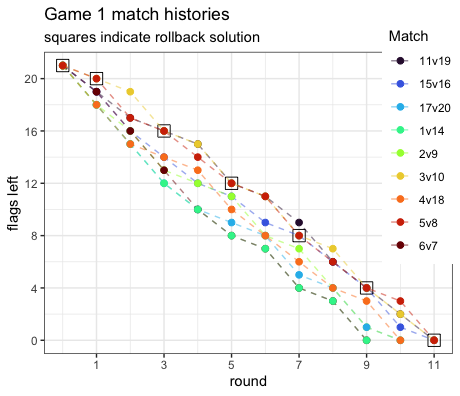
\includegraphics[width=.6\linewidth]{figures/Game1.png} 
% \end{figure}
%
% \begin{figure}[!h]
%   \centering
%   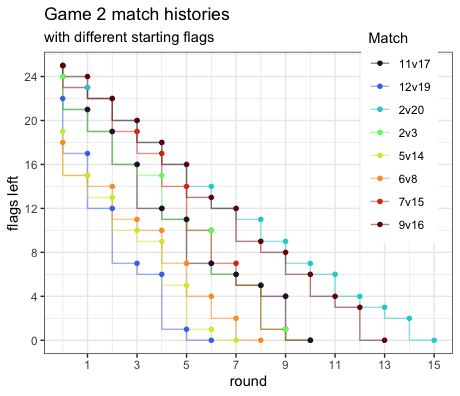
\includegraphics[width=.6\linewidth]{figures/Game2.png} 
% \end{figure}

%------------------------------------------------------------------%

% \question[20] 
% The countries of Oceania and Eurasia are at war.
% As depicted in the figure, Oceania has four cities —
% Argula, Betra, Carnat, and Dussel — 
% and it is concerned that one of them is to be bombed by Eurasia.
% The bombers could come from either base Alpha,
% which can reach the cities of Argula and Betra;
% or from base Beta, which can reach either Carnat or Dussel.
% Eurasia decides which one of these four cities to attack.
% Oceania doesn’t know which one has been selected,
% but does observe the base from which the bombers are flying.
% After making that observation, Oceania decides which one 
% (and only one) of its four cities to evacuate.
%
% Assign a payoff of 2 to Oceania
% if it succeeds in evacuating the city that is to be bombed
% and a payoff of 1 otherwise.
% Assign Eurasia a payoff of 1 if the city it bombs was not evacuated
% and a zero payoff otherwise.
% Write down the extensive form game.
% \footnote{Harrington \textit{Games, Strategies, and Decision Making}}
%
% %\vspace{-5cm}
% \begin{figure}[!h]
%   \centering
%   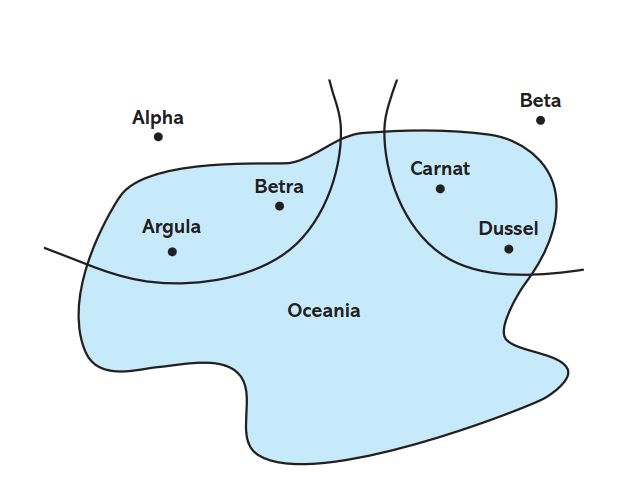
\includegraphics[width=.3\linewidth]{figures/figPR2.1.png} 
% \end{figure}
%
% \begin{solution}
%   \begin{center}
%     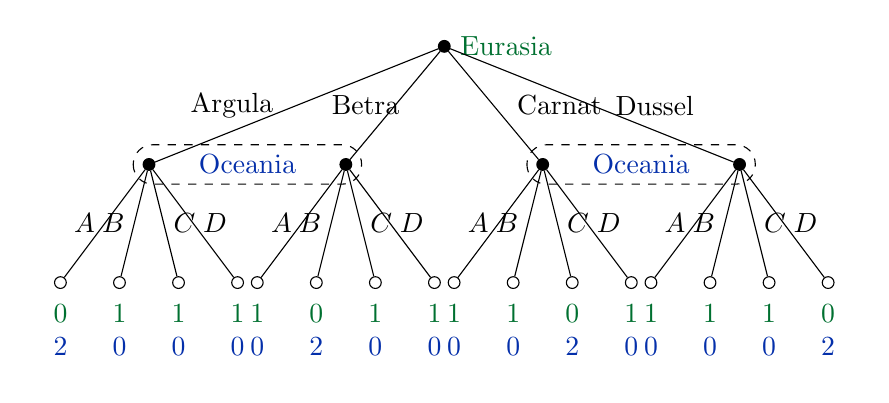
\begin{tikzpicture}[
% font=\footnotesize
]
    \tikzstyle{solid node}=[circle,draw,inner sep=1.5,fill=black]
    \tikzstyle{hollow node}=[circle,draw,inner sep=1.5]
    \tikzstyle{level 1}=[level distance=15mm,sibling distance=2.5cm]
    \tikzstyle{level 2}=[level distance=15mm,sibling distance=.75cm]
    \tikzstyle{level 3}=[level distance=15mm,sibling distance=0.5cm]
    
    \node(0)[solid node,label=right:{\color{ducksgreen} Eurasia}]{}
        child{node(1)[solid node,label=above left:{ }]{}
            child{node[hollow node,label=below:{
                \begin{tabular}{c}
                     {\color{ducksgreen} 0}  \\
                     {\color{darkblue} 2} 
                \end{tabular}
            }]{} edge from parent node[left]{$A$}}
            child{node[hollow node,label=below:{
                \begin{tabular}{c}
                     {\color{ducksgreen} 1}  \\
                     {\color{darkblue} 0} 
                \end{tabular}
            }]{} edge from parent node[left]{$B$}}
            child{node[hollow node,label=below:{
                \begin{tabular}{c}
                     {\color{ducksgreen} 1}  \\
                     {\color{darkblue} 0} 
                \end{tabular}
            }]{} edge from parent node[right]{$C$}}
            child{node[hollow node,label=below:{
                \begin{tabular}{c}
                     {\color{ducksgreen} 1}  \\
                     {\color{darkblue} 0} 
                \end{tabular}
            }]{} edge from parent node[right]{$D$}}
            edge from parent node[left,xshift=-5]{Argula}
        }
        child{node(2)[solid node,label=above right:{ }]{}
            child{node[hollow node,label=below:{
                \begin{tabular}{c}
                     {\color{ducksgreen} 1}  \\
                     {\color{darkblue} 0} 
                \end{tabular}
            }]{} edge from parent node[left]{$A$}}
            child{node[hollow node,label=below:{
                \begin{tabular}{c}
                     {\color{ducksgreen} 0}  \\
                     {\color{darkblue} 2} 
                \end{tabular}
            }]{} edge from parent node[left]{$B$}}
            child{node[hollow node,label=below:{
                \begin{tabular}{c}
                     {\color{ducksgreen} 1}  \\
                     {\color{darkblue} 0} 
                \end{tabular}
            }]{} edge from parent node[right]{$C$}}
            child{node[hollow node,label=below:{
                \begin{tabular}{c}
                     {\color{ducksgreen} 1}  \\
                     {\color{darkblue} 0} 
                \end{tabular}
            }]{} edge from parent node[right]{$D$}}
            edge from parent node[left,xshift=5]{Betra}
        }
        child{node(3)[solid node,label=above right:{ }]{}
            child{node[hollow node,label=below:{
                \begin{tabular}{c}
                     {\color{ducksgreen} 1}  \\
                     {\color{darkblue} 0} 
                \end{tabular}
            }]{} edge from parent node[left]{$A$}}
            child{node[hollow node,label=below:{
                \begin{tabular}{c}
                     {\color{ducksgreen} 1}  \\
                     {\color{darkblue} 0} 
                \end{tabular}
            }]{} edge from parent node[left]{$B$}}
            child{node[hollow node,label=below:{
                \begin{tabular}{c}
                     {\color{ducksgreen} 0}  \\
                     {\color{darkblue} 2} 
                \end{tabular}
            }]{} edge from parent node[right]{$C$}}
            child{node[hollow node,label=below:{
                \begin{tabular}{c}
                     {\color{ducksgreen} 1}  \\
                     {\color{darkblue} 0} 
                \end{tabular}
            }]{} edge from parent node[right]{$D$}}
            edge from parent node[right,xshift=5]{Carnat}
        }
        child{node(4)[solid node,label=above right:{ }]{}
            child{node[hollow node,label=below:{
                \begin{tabular}{c}
                     {\color{ducksgreen} 1}  \\
                     {\color{darkblue} 0} 
                \end{tabular}
            }]{} edge from parent node[left]{$A$}}
            child{node[hollow node,label=below:{
                \begin{tabular}{c}
                     {\color{ducksgreen} 1}  \\
                     {\color{darkblue} 0} 
                \end{tabular}
            }]{} edge from parent node[left]{$B$}}
            child{node[hollow node,label=below:{
                \begin{tabular}{c}
                     {\color{ducksgreen} 1}  \\
                     {\color{darkblue} 0} 
                \end{tabular}
            }]{} edge from parent node[right]{$C$}}
            child{node[hollow node,label=below:{
                \begin{tabular}{c}
                     {\color{ducksgreen} 0}  \\
                     {\color{darkblue} 2} 
                \end{tabular}
            }]{} edge from parent node[right]{$D$}}
            edge from parent node[right,xshift=5]{Dussel}
        };

    % information set
    \draw[dashed,rounded corners=7]($(1)+(-.2,.25)$)rectangle($(2)+(.2,-.25)$);
    \draw[dashed,rounded corners=7]($(3)+(-.2,.25)$)rectangle($(4)+(.2,-.25)$);
    % specify movers
    \node at ($.5*(1)+.5*(2)$) {\color{darkblue} Oceania};
    \node at ($.5*(3)+.5*(4)$) {\color{darkblue} Oceania};
\end{tikzpicture}
 
%   \end{center} 
%
%   Note that $A$, $B$, $C$, and $D$ in the last row are short for the city names.
%   Eurasia acts first, so the initial node is labelled accordingly.
%   Oceania has only two info sets which are represented with the dashed ovals.
%   The $(0,2)$ or $(1,0)$ payoff sets correspond to Oceania choosing the same city that is bombed,
%   or choosing a different city respectively.
% \end{solution}
%
% \newpage

%------------------------------------------------------------------

\end{questions}

\end{document}
